
% Thiên Lộc


\section{Architecture Overview}

\subsection {Moodle diagram}
\begin{figure}[H]
    \centering
    % Placeholder: insert system architecture diagram image here
    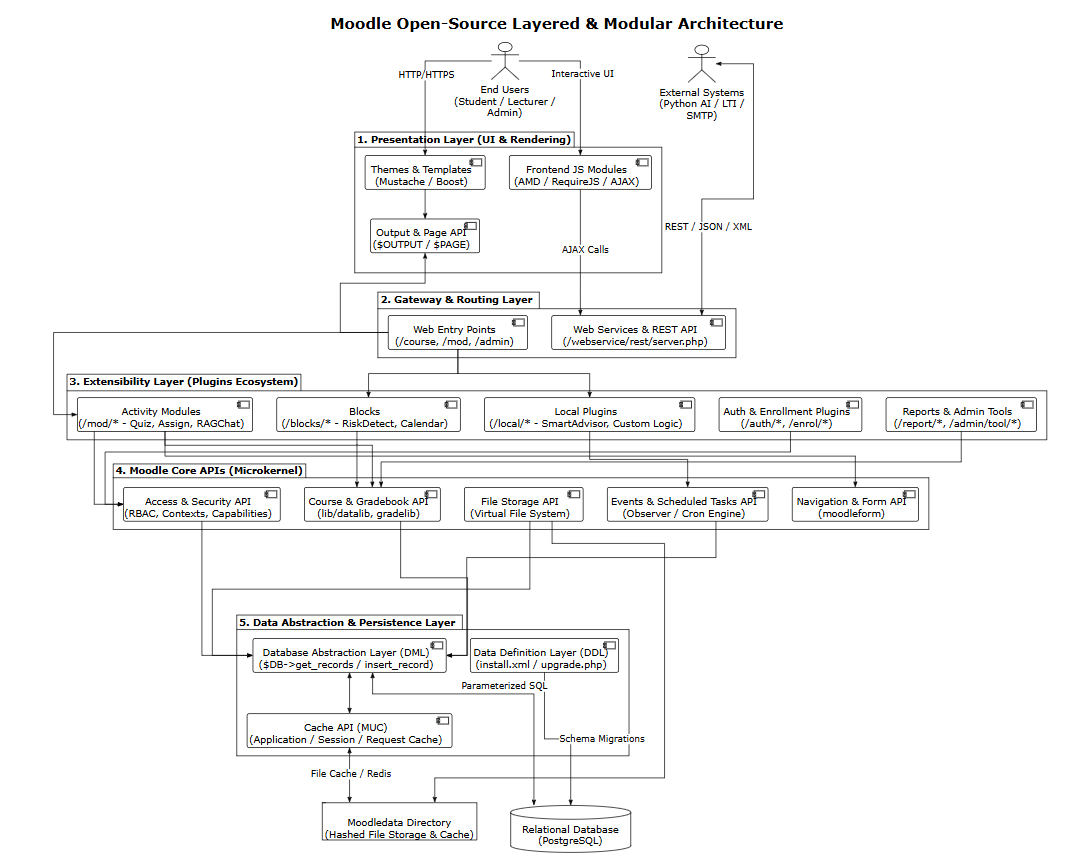
\includegraphics[width=0.85\textwidth, keepaspectratio]{images/architecture_diagram/moodle-diagram.png}
    \caption{Moodle Diagram}
    \label{fig:moodle-diagram}
\end{figure}

Moodle follows a layered and modular architecture that separates the user interface (presentation) from the underlying business logic. The presentation layer is responsible for managing the visual aspects of the system through themes and templates. Additionally, rendering components generate HTML pages based on data provided by the application logic and underlying domain models.

Moodle is structured around a central application core (Moodle Core), which is surrounded by an extensible ecosystem of plugins. This design allows developers to introduce new functionalities without directly modifying the core libraries and components. Moodle Core provides the fundamental infrastructure required to build and operate a Learning Management System (LMS). It implements essential functionalities that all plugins rely on, including:


\begin{itemize}
    \item \textbf{Courses \& Activities:} A Moodle course consists of a collection of learning activities and resources organized into sections. Courses are structured within a hierarchical category system and displayed through the Moodle web interface.

    \item \textbf{Users:} Users are individuals who interact with the Moodle platform, including students, lecturers, and administrators. Each user is assigned specific roles and permissions that determine their level of access to system functionalities.

    \item \textbf{Course Enrolment:} The enrolment mechanism allows users to participate in courses under specific roles, such as students or teachers. It manages course registration and determines users' access to course-related resources and activities.

    \item \textbf{Access Control \& Security:} Moodle provides role-based access control (RBAC) to manage permissions and restrict access to system resources based on user roles and capabilities.

    \item \textbf{Gradebook:} Moodle provides grade management functionalities that allow lecturers to evaluate student performance, manage grades, and track learning progress.

    \item \textbf{File Management:} Moodle provides a centralized file storage mechanism for managing course materials, user uploads, and other resources through its file storage API.

    \item \textbf{Events \& Scheduled Tasks:} Moodle supports event-driven operations and scheduled background tasks to handle automated processes and system activities.
\end{itemize}


In addition to these core functionalities, Moodle supports various plugin types, such as Activity Modules, Blocks, Local Plugins, Authentication Plugins, and Reporting Plugins. These plugins extend the platform's capabilities while reusing the services provided by Moodle Core.
\subsection {Overall architecture diagram}
\begin{figure}[H]
    \centering
    % Placeholder: insert system architecture diagram image here
    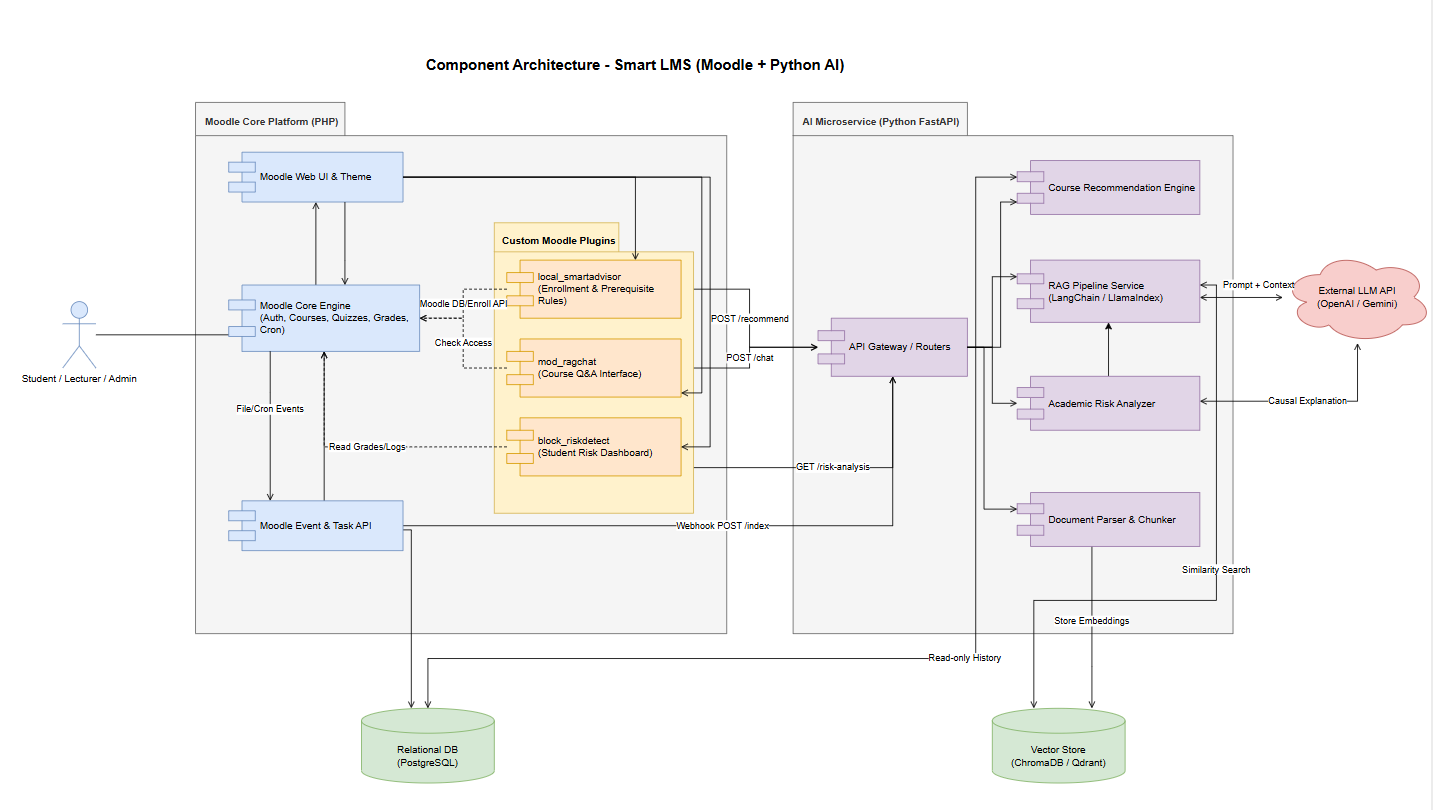
\includegraphics[width=0.85\textwidth, keepaspectratio]{images/architecture_diagram/component-diagram.png}
    \caption{Overall System Architecture Diagram}
    \label{fig:arch-overview}
\end{figure}

Figure~\ref{fig:arch-overview} illustrates the high-level Component Architecture of the proposed Intelligent Learning Management System (Smart LMS). The system adopts a hybrid modular architecture that decouples core academic administration from computationally intensive Artificial Intelligence (AI) workloads. By bridging an open-source Moodle core with an independent Python-based AI microservice via RESTful APIs, the design ensures high maintainability, scalability, and separation of concerns.